\باب{درجہ دوم سادہ تفرقی مساوات}
کئی اہم میکانی اور برقی مسائل کو خطی دو درجی تفرقی مساوات سے ظاہر کیا جا سکتا ہے۔خطی دو درجی تفرقی مساوات  تمام خطی تفرقی مساوات کی نمائندگی کرتا ہے۔چونکہ دو درجی مساوات کا حل نسبتاً آسان ہوتا ہے لہٰذا اس باب میں اسی پر پہلے غور کرتے ہیں۔اگلے باب کا موضوع تین درجی مساوات ہے۔

تفرقی مساوات کو خطی اور غیر خطی گروہوں میں تقسیم کیا جاتا ہے۔غیر خطی تفرقی مساوات کے حل کا حصول مشکل ثابت ہوتا ہے جبکہ خطی مساوات حل کرنے کے کئی عمدہ ترکیب پائے جاتے ہیں۔اس باب میں عمومی حل اور ابتدائی معلومات کی صورت میں جبری حل کا حصول دکھایا جائے گا۔

\حصہ{متجانس خطی دو درجی تفرقی مساوات}
یک درجی مساوات پر پہلے باب میں غور کیا گیا۔اس باب میں دو درجی مساوات پر غور کیا جائے گا۔یہ مساوات میکانی اور برقی \اصطلاح{ارتعاش}\فرہنگ{ارتعاش}\حاشیہب{oscillations}\فرہنگ{oscillations}، متحرک امواج، منتقلی حرارتی توانائی اور طبیعیات کے دیگر شعبوں میں کلیدی کردار ادا کرتے ہیں۔

ایسا دو درجی تفرقی مساوات جس کو
\begin{align}\label{مساوات_سادہ_دو_درجی_تعریف}
y''+p(x)y'+q(x)y=r(x)
\end{align}
صورت میں لکھا جا سکے \اصطلاح{خطی}\فرہنگ{خطی!دو درجی}\حاشیہب{linear}\فرہنگ{linear!second order} کہلاتا ہے ورنہ اس کو \اصطلاح{غیر خطی}\فرہنگ{غیر خطی}\حاشیہب{nonlinear}\فرہنگ{nonlinear} کہتے ہیں۔

اس مساوات کی خاصیت یہ ہے کہ اس میں \عددی{y}، \عددی{y'} اور \عددی{y''} کی طاقت اکائی ہے  یعنی تینوں خطی ہیں البتہ \عددی{p(x)}، \عددی{q(x)} اور \عددی{r(x)} متغیرہ \عددی{x} کے کوئی بھی تفاعل ہو سکتے ہیں۔دو درجی مساوات کا پہلا جزو \عددی{f(x)y''} ہونے کی صورت میں مساوات کو \عددی{f(x)} سے تقسیم کرتے ہوئے اس کو مساوات \حوالہ{مساوات_سادہ_دو_درجی_تعریف} کی \اصطلاح{معیاری صورت}\فرہنگ{معیاری صورت!دو درجی}\حاشیہب{standard form}\فرہنگ{standard form!second order} میں لکھیں جہاں  \عددی{y''} پہلا  جزو ہے۔

متجانس اور غیر متجانس دو درجی مساوات کی تعریف ہو بہو ایک درجی متجانس اور غیر متجانس مساوات کی تعریف کی طرح ہے جس پر حصہ \حوالہ{حصہ_سادہ_اول_متجانس_خطی} میں تبصرہ کیا گیا۔یقیناً \عددی{r \equiv 0} [جہاں زیر غور تمام \عددی{x} پر  \عددی{r(x)=0} ہو؛ اس کو \اصطلاح{مکمل صفر}\فرہنگ{مکمل صفر}\حاشیہب{identically zero}\فرہنگ{identically zero} پڑھیں۔] کی صورت میں مساوات \حوالہ{مساوات_سادہ_دو_درجی_تعریف} درج ذیل لکھی جائے گی 
\begin{align}\label{مساوات_سادہ_متجانس_دو_درجی_تعریف}
y''+p(x)y'+q(x)y=0
\end{align}
جو \اصطلاح{متجانس} ہے۔اگر \عددی{r(x) \not\equiv 0} ہو تب مساوات \حوالہ{مساوات_سادہ_دو_درجی_تعریف} \اصطلاح{غیر متجانس}\فرہنگ{غیر متجانس!دو درجی}\حاشیہب{nonhomogenous}\فرہنگ{nonhomogenous!second order} کہلائے گا۔

متجانس خطی تفرقی مساوات کی مثال درج ذیل ہے
\begin{align*}
xy''+2y'+y=0,\quad \text{\RL{ جو کو معیاری صورت میں لکھتے ہیں}} \quad y''+\frac{2y'}{x}+\frac{y}{x}=0
\end{align*}
جبکہ غیر متجانس خطی تفرقی مساوات کی مثال
\begin{align*}
y''+x^2y=\sec x
\end{align*}
ہے۔آخر میں غیر خطی مساوات کی تین مثال پیش کرتے ہیں۔
\begin{align*}
\left(y''\right)^3+xy=\sin x, \quad y''+xy'+4y^2=0, \quad yy''-xy'=0
\end{align*}
تفاعل \عددی{p} اور \عددی{q} مساوات \حوالہ{مساوات_سادہ_متجانس_دو_درجی_تعریف} کے \اصطلاح{عددی سر}\فرہنگ{عددی سر!دو درجی مساوات}\حاشیہب{coefficients}\فرہنگ{coefficients} کہلاتے ہیں۔

دو درجی مساوات کے حل کی تعریف عین ایک درجی مساوات کے حل کی مانند ہے۔ تفاعل \عددی{y=h(x)} کو کھلے وقفہ \عددی{I} پر اس صورت خطی (یا غیر خطی) دو درجی تفرقی مساوات کا حل تصور کیا جاتا ہے جب اس پورے فاصلے پر \عددی{h(x)}، \عددی{h'} اور \عددی{h''}  پائے جاتے ہوں اور  تفرقی مساوات میں \عددی{y} کی جگہ \عددی{h}، \عددی{y'} کی جگہ \عددی{h'} اور \عددی{y''} کی جگہ \عددی{h''} پر کرنے سے مساوات کے دونوں اطراف بالکل یکساں صورت اختیار کرتے ہوں۔چند مثال جلد پیش کرتے ہیں۔
%==========================

\حصہء{متجانس خطی تفرقی مساوات}
اس باب کے پہلے حصے میں متجانس خطی مساوات پر غور کیا جائے گا جبکہ بقایا باب میں غیر متجانس خطی مساوات پر غور کیا جائے گا۔ 

خطی تفرقی مساوات حل کرنے کے نہایت عمدہ تراکیب پائے جاتے ہیں۔متجانس مساوات کے حل میں \اصطلاح{اصول خطیت}\فرہنگ{اصول!خطیت}\فرہنگ{خطیت!اصول}\حاشیہب{linearity principle}\فرہنگ{linearity!principle} یا \اصطلاح{اصول نفاذ}\فرہنگ{اصول!نفاذ}\فرہنگ{نفاذ!اصول}\حاشیہب{superposition principle}\فرہنگ{superposition!principle} کلیدی کردار ادا کرتا ہے جس کے تحت متجانس مساوات کے مختلف حل کو آپس میں جمع کرنے یا انہیں مستقل سے ضرب دینے سے دیگر حل حاصل کئے جا سکتے ہیں۔
%===================

\ابتدا{مثال}\شناخت{مثال_سادہ_دو_درجی_اصول_نفاذ}\quad اصول نفاذ\\
تمام \عددی{x} پر درج ذیل متجانس خطی تفرقی مساوات کے حل \عددی{y_1=\cos 2x} اور \عددی{y_2=\sin 2x} ہیں۔
\begin{align}
y''+4y=0
\end{align}
ان حل کی درستگی ثابت کرنے کی خاطر انہیں دیے گئے مساوات میں پر کرتے ہیں۔پہلے \عددی{y_1=\cos 2x} کو درست حل ثابت کرتے ہیں۔چونکہ \عددی{(\cos 2x)''=-4\cos 2x} کے برابر ہے لہٰذا 
\begin{align*}
y''+4y=(\cos 2x)''+4(\cos 2x)=-4\cos 2x+4\cos 2x=0
\end{align*}
ملتا ہے۔اسی طرح \عددی{y_2=\sin 2x} کو پر کرتے ہوئے 
\begin{align*}
y''+4y=(\sin 2x)''+4(\sin 2x)=-4\sin 2x+4\sin 2x=0
\end{align*}
ملتا ہے۔ہم دیے گئے حل سے نئے حل حاصل کر سکتے ہیں۔یوں ہم \عددی{\cos 2x} کو کسی مستقل مثلاً \عددی{2.73} سے ضرب دیتے ہوئے اور \عددی{\sin 2x} کو  \عددی{-1.25} سے ضرب دیتے ہوئے ان کا مجموعہ
\begin{align*}
y_3=2.73\cos 2x-1.25\sin 2x
\end{align*}
لیتے ہوئے  توقع کرتے ہیں کہ یہ بھی دیے گئے تفرقی مساوات کا حل ہو گا۔آئیں نئے حل کو تفرقی مساوات میں پر کرتے ہوئے اس کی درستگی ثابت کریں۔
\begin{align*}
y''+4y&=(2.73\cos 2x-1.25\sin 2x)''+4(2.73\cos 2x-1.25\sin 2x)\\
&=4(-2.73\cos 2x+1.25\sin 2x)+4(2.73\cos 2x-1.25\sin 2x)\\
&=0
\end{align*}
\انتہا{مثال}
%=======================

اس مثال میں ہم نے دیے گئے حل \عددی{y_1} اور \عددی{y_2} سے نیا حل 
\begin{align}
y_3=c_1 y_1+c_2 y_2, \quad \text{\RL{($c_1$\, اور \, $c_2$\,اختیاری مستقل ہیں)}}
\end{align}
حاصل کیا۔ اس کو \عددی{y_1} اور \عددی{y_2} کا \اصطلاح{خطی میل}\فرہنگ{خطی!میل}\حاشیہب{linear combination}\فرہنگ{linear!combination} کہتے ہیں۔اس مثال سے ہم \اصطلاح{مسئلہ خطی میل}\فرہنگ{مسئلہ!خطی میل} بیان کرتے ہیں جسے عموماً \اصطلاح{اصول خطیت}\فرہنگ{اصول!خطیت} یا \اصطلاح{اصول نفاذ}\فرہنگ{اصول نفاذ} کہا جاتا ہے۔

%======================================

\ابتدا{مسئلہ}\شناخت{مسئلہ_دو_درجی_خطی_میل}\quad مسئلہ خطی میل\\
کھلے وقفہ \عددیء{I} پر متجانس خطی دو درجی تفرقی مساوات کے دو عدد حل کا خطی میل بھی \عددیء{I} پر اس مساوات کا حل ہو گا۔بالخصوص ان حل کو مستقل مقدار سے ضرب دینے سے بھی مساوات کے حل حاصل ہوتے ہیں۔
\انتہا{مسئلہ}

ثبوت: تصور کریں کہ متجانس مساوات \حوالہ{مساوات_سادہ_متجانس_دو_درجی_تعریف} کے دو حل \عددی{y_1} اور \عددی{y_2} پائے جاتے ہیں لہٰذا
\begin{gather}
\begin{aligned}\label{مساوات_درجہ_دو_خطی_میل}
y_1''+py_1'+qy_1&=0\\
y_2''+y_2'+qy_2&=0
\end{aligned}
\end{gather}
ہو گا۔خطی میل سے نیا حل \عددی{y_3=c_1 y_1+c_2 y_2} حاصل کرتے ہیں۔اس کا ایک درجی تفرق اور دو درجی تفرق درج ذیل ہیں۔
\begin{align*}
y_3' &=c_1y_1'+c_2y_2'\\
y_3'' &=c_1 y_1''+c_2y_2''
\end{align*}
\عددی{y_3}، \عددی{y_3'} اور \عددی{y_3''} کو متجانس مساوات کے بائیں ہاتھ میں پر کرتے ہیں
\begin{align*}
y_3''+py_3'+qy_3&=(c_1 y_1''+c_2y_2'')+p(c_1y_1'+c_2y_2')+q(c_1 y_1+c_2 y_2)\\
&=c_1(y_1''+py_1'+qy_1)+c_2(y_2''+py_2'+qy_2)\\
&=0
\end{align*}
جہاں مساوات \حوالہ{مساوات_درجہ_دو_خطی_میل} سے آخری قدم پر دونوں قوسین صفر کے برابر پر کئے گئے ہیں۔یوں مساوات کا بایاں ہاتھ اور دایاں ہاتھ برابر ہیں لہٰذا ثابت ہوتا ہے کہ \عددی{y_3} بھی مساوات   \حوالہ{مساوات_سادہ_متجانس_دو_درجی_تعریف} کا حل ہے۔

یہاں یاد رہے کہ مسئلہ \حوالہ{مسئلہ_دو_درجی_خطی_میل} صرف متجانس مساوات کے لئے قابل استعمال ہے۔غیر متجانس مساوات کے دیگر حل اس مسئلے سے حاصل نہیں کئے جا سکتے ہیں۔
%======================================

\ابتدا{مثال}
تصور کریں کہ \عددی{y_1} اور \عددی{y_2} غیر متجانس مساوات \حوالہ{مساوات_سادہ_دو_درجی_تعریف} کے حل ہیں۔ثابت کریں کہ \عددی{y_3=c_1y_1+c_2y_2} اس متجانس مساوات کا حل نہیں ہے جہاں \عددی{c_1} اور \عددی{c_2} مستقل مقدار ہیں۔

حل:\عددی{y_1} اور \عددی{y_2} غیر متجانس مساوات کے حل ہیں لہٰذا انہیں متجانس مساوات میں پر کرنے سے مساوات کے دونوں اطراف برابر حاصل ہوتے ہیں یعنی
\begin{gather}
\begin{aligned}\label{مساوات_سادہ_دو_درجی_غیر_متجانس_حل_الف}
y_1''+py_1'+qy_1&=r\\
y_2''+py_2'+qy_2&=r
\end{aligned}
\end{gather}
\عددی{y_3} کو مساوات کے بائیں ہاتھ میں پر کرتے ہیں
\begin{align*}
y_3''+py'+qy&=(c_1y_1+c_2y_2)''+p(c_1y_1+c_2y_2)'+q(c_1y_1+c_2y_2)\\
&=(c_1y_1''+c_2y_2'')+p(c_1y_1'+c_2y_2')+q(c_1y_1+c_2y_2)\\
&=c_1(y_1''+py_1'+qy_1)+c_2(y_2''+py_2'+qy_2)\\
&=(c_1+c_2)r
\end{align*}
 جہاں آخری قدم پر مساوات \حوالہ{مساوات_سادہ_دو_درجی_غیر_متجانس_حل_الف} کا استعمال کیا گیا۔اس سے \عددی{(c_1+c_2)r} حاصل ہوتا ہے جبکہ متجانس مساوات کا دایاں ہاتھ \عددی{r} کے برابر ہے لہٰذا \عددی{y_3} متجانس مساوات پر پورا نہیں اترتا۔یوں \عددی{y_3} متجانس مساوات کا حل نہیں ہے۔
\انتہا{مثال}
%=====================================
\ابتدا{مشق}\quad غیر متجانس خطی مساوات\\
درج ذیل خطی غیر متجانس مساوات میں \عددی{y=2-\cos x} اور \عددی{y=2-\sin x} کو پر کرتے ہوئے ثابت کریں کہ یہ مساوات کے حل ہیں۔ثابت کریں کہ ان کا مجموعہ مساوات کا حل نہیں ہے۔اسی طرح ثابت کریں کہ \عددی{3(2-\cos x)} یا \عددی{-7(2-\sin x)} بھی مساوات کے حل نہیں ہیں۔
\begin{align*}
y''+y=2
\end{align*}

\انتہا{مشق}
%==================================
\ابتدا{مشق}
درج ذیل مساوات میں \عددی{y=1} اور \عددی{y=x^3} پر کرتے ہوئے ثابت کریں کہ یہ دونوں تفرقی مساوات کے حل ہیں۔ثابت کریں کہ ان کا مجموعہ تفرقی مساوات کا حل نہیں ہے نا ہی \عددی{y=-x^3} حل ہے۔اس کا مطلب یہ ہوا کہ حل کو \عددی{-1} سے بھی ضرب دے کر نیا حل نہیں حاصل کیا جا سکتا ہے۔
\begin{align*}
yy''-2x^2y'=0
\end{align*}
\انتہا{مشق}
%=================================

\حصہء{ابتدائی قیمت مسائل۔ اساس۔ عمومی حل}
باب \حوالہ{باب_سادہ_اول_تفرقی} میں ابتدائی قیمت درجہ اول سادہ تفرقی مساوات پر غور کیا گیا۔درجہ اول سادہ تفرقی مساوات اور ابتدائی معلومات \عددی{y(x_0)=y_0} مل کر ابتدائی قیمت تفرقی مساوات کہلاتے ہیں۔ابتدائی قیمت کو استعمال کرتے ہوئے درجہ اول سادہ تفرقی مساوات کے عمومی حل کا واحد اختیاری مستقل \عددی{c} حاصل کرتے ہوئے جبری یکتا حل حاصل کیا جاتا ہے۔اسی تصور کو دو درجی سادہ تفرقی مساوات تک بڑھاتے ہیں۔

دو درجی متجانس خطی ابتدائی قیمت مسئلے سے مراد متجانس مساوات \حوالہ{مساوات_سادہ_متجانس_دو_درجی_تعریف} اور درج ذیل ابتدائی معلومات ہیں۔
\begin{align}\label{مساوات_سادہ_دو_درجی_ابتدائی_قیمتیں}
y(x_0)=K_0,\quad y'(x_0)=K_1
\end{align}
\عددی{K_0} اور \عددی{K_1}  کھلے وقفہ پر نقطہ \عددی{x_0} پر بالترتیب نقطہ عمومی حل اور حل کے تفرق (یعنی ڈھلوان) کی قیمتیں ہیں۔ 

مساوات \حوالہ{مساوات_سادہ_دو_درجی_ابتدائی_قیمتیں} میں دیے گئے ابتدائی قیمتوں سے عمومی حل
\begin{align}
y=c_1y_1+c_2y_2
\end{align}
کے اختیاری مستقل \عددی{c_1} اور \عددی{c_2} کی قیمتیں حاصل کی جاتی ہیں۔یہاں \عددی{y_1} اور \عددی{y_2} مساوات \حوالہ{مساوات_سادہ_دو_درجی_ابتدائی_قیمتیں} کے حل ہیں۔یوں جبری حل حاصل کیا جاتا ہے جو نقطہ \عددی{(x_0,K_0)} سے گزرتا ہے اور جس کی ڈھلوان اس نقطے پر \عددی{K_1} ہوتی ہے۔
%==============

\ابتدا{مثال}\شناخت{مثال_سادہ_دو_درجی_ابتدائی_قیمت_الف}
درج ذیل ابتدائی قیمت دو درجی سادہ تفرقی مساوات کو حل کریں۔
\begin{align*}
y''+4y=0,\quad y(0)=5,\quad y'(0)=-3
\end{align*}

حل:پہلا قدم: اس مساوات کے حل  \عددی{y_1=\cos 2x} اور \عددی{y_2=\sin 2x} ہیں (مثال \حوالہ{مثال_سادہ_دو_درجی_اصول_نفاذ} سے رجوع کریں) لہٰذا اس کا موزوں عمومی حل
\begin{align}\label{مساوات_سادہ_دو_درجی_عمومی_حل_الف}
y=c_1\cos 2x+c_2\sin 2x
\end{align}
ہو گا۔ (موزوں حل پر اس مثال کے فوراً بعد بات کرتے ہیں۔)

دوسرا قدم:جبری حل حاصل کرتے ہیں۔عمومی حل کا تفرق \عددی{y'=-2\sin 2x +2c_2\cos x} ہے۔ابتدائی قیمتیں استعمال کرتے ہوئے
\begin{align*}
y(0)&=c_1 \cos 0+c_2\sin 0=c_1=5\\
y'(0)&=-2\sin 0+2c_2\cos 0=2c_2=-3, \quad c_2=-1.5
\end{align*}
حاصل ہوتے ہیں لہٰذا جبری حل
\begin{align*}
y=5\cos 2x-1.5\sin 2x
\end{align*}
ہو گا۔شکل \حوالہ{شکل_مثال_سادہ_دو_درجی_ابتدائی_قیمت_الف} میں جبری حل دکھایا گیا ہے۔نقطہ \عددی{x=0} پر اس کی قیمت \عددی{y(0)=5} ہے جبکہ اسی نقطے پر خط کی ڈھلوان (مماس) \عددی{y'(0)=0.5} ہے۔مماس \عددی{x} محور کو \عددی{x=\tfrac{5}{3}=3.33} پر قطع کرتا ہے۔
\begin{figure}
\centering
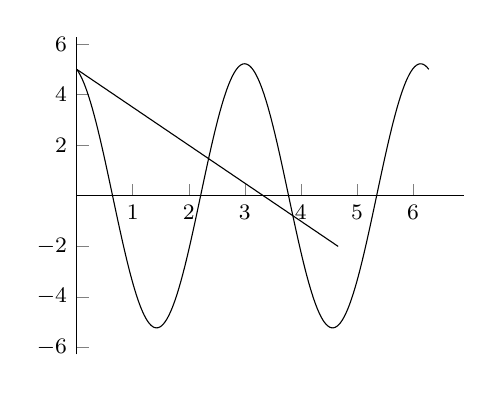
\begin{tikzpicture}
\begin{axis}[small,axis lines*=middle,xmin=0]
\addplot[domain=0:2*pi,samples=200]{5*cos(2*x*180/pi)-1.5*sin(2*x*180/pi)};
\addplot[] plot coordinates {(0,5) (4.666,-2)};
\end{axis}
\end{tikzpicture}
\caption{مثال \حوالہ{مثال_سادہ_دو_درجی_ابتدائی_قیمت_الف} کا جبری حل۔}
\label{شکل_مثال_سادہ_دو_درجی_ابتدائی_قیمت_الف}
\end{figure}
\انتہا{مثال}
%===================

درج بالا مثال میں \عددی{y_1} اور \عددی{y_2} ایسے تفاعل تھے جن سے حاصل عمومی حل ابتدائی معلومات پر پورا اترتا تھا۔آئیں اب دو آپس میں راست تناسب حل لیتے ہوئے عمومی حل  لکھیں، مثلاً \عددی{y_1=\cos 2x} اور \عددی{y_2=k\cos 2x} لیتے ہوئے
\begin{align*}
y=c_1\cos 2x+c_2 k\cos 2x=(c_1+c_2k)\cos 2x=c_3\cos 2x
\end{align*}
عمومی حل لکھتے ہیں۔اس مساوات میں ایک عدد اختیاری مستقل \عددی{c_3} پایا جاتا ہے جو دونوں ابتدائی قیمتوں پر پورا اترنے کے لئے نا کافی ہے۔یوں ہم دیکھتے ہیں کہ عمومی حل لکھتے ہوئے ایسے موزوں حل کا خطی میل لیا جاتا ہے جو آپس میں راست تناسبی نہ ہوں۔

 آپ نے یہ بھی دیکھ لیا ہو گا کہ عمومی حل میں استعمال ہونے والے موزوں حل \عددی{y_1} اور \عددی{y_2} انفرادی طور پر دونوں ابتدائی معلومات پر پورا نہیں اتر سکتے البتہ ان کا خطی میل دونوں ابتدائی معلومات پر پورا اترتا ہے۔یہی عمومی حل کی اہمیت کی وجہ ہے۔
%===========================

\ابتدا{قانون}\quad عمومی حل، اساس اور جبری حل کے تعریف\\
کھلے وقفہ \عددی{I} پر سادہ تفرقی مساوات \حوالہ{مساوات_سادہ_متجانس_دو_درجی_تعریف} کا عمومی حل مساوات \حوالہ{مساوات_سادہ_دو_درجی_عمومی_حل_الف} دیتا ہے جہاں \عددی{I} پر \عددی{y_1} اور \عددی{y_2} مساوات  \حوالہ{مساوات_سادہ_متجانس_دو_درجی_تعریف} کے  (آپس میں) غیر تناسبی حل اور \عددی{c_1}، \عددی{c_2} اختیاری مستقل ہیں۔فاصلہ \عددی{I} پر \عددی{y_1} اور \عددی{y_2} مساوات \حوالہ{مساوات_سادہ_متجانس_دو_درجی_تعریف} کی \اصطلاح{اساس}\فرہنگ{اساس!حل}\حاشیہب{basis}\فرہنگ{basis!of solutions} حل کہلاتے ہیں۔

کھلے وقفہ \عددی{I} پر سادہ تفرقی مساوات \حوالہ{مساوات_سادہ_متجانس_دو_درجی_تعریف} کا جبری حل مساوات \حوالہ{مساوات_سادہ_دو_درجی_عمومی_حل_الف} میں \عددی{c_1} اور \عددی{c_2} کی جگہ مخصوص قیمتیں پر کرنے سے حاصل ہوتا ہے۔
\انتہا{قانون}
%============================

کھلے وقفہ کی تعریف حصہ \حوالہ{حصہ_حل_کا_تصور_سادہ_اول} میں دی گئی ہے۔ \عددی{y_1} اور \عددی{y_2} اس صورت  تناسبی تصور کئے جاتے ہیں  جب پورے \عددی{I} پر
\begin{align}
(a)\quad y_1=ky_2 \quad \text{یا} \quad  (b) \quad y_2=ly_1
\end{align} 
ہو، جہاں \عددی{k} اور \عددی{l} اعداد ہیں جو صفر بھی ہو سکتے ہیں۔(یہاں توجہ رکھیں: \عددی{a} اس صورت \عددی{b} کے مترادف ہے جب \عددی{k \ne 0} ہو۔)

آئیں اساس کی تعریف ذرہ مختلف اور عمومی اہمیت کے حامل طریقے سے بیان کریں۔  وقفہ \عددی{I} پر معین \عددی{y_1} اور \عددی{y_2} اس وقفے پر اس صورت \اصطلاح{خطی طور غیر تابع}\فرہنگ{خطی طور! غیر تابع}\حاشیہب{linearly independent}\فرہنگ{linearly independent} کہلاتے ہیں جب پورے \عددی{I} پر
\begin{align}\label{مساوات_سادہ_دو_درجی_خطی_طور_غیر_تابع_الف}
k_1 y_1+k_2 y_2=0
\end{align}
سے مراد 
\begin{gather}
\begin{aligned}
k_1&=0\\
k_2&=0
\end{aligned}
\end{gather}
ہو۔\عددی{k_1} اور \عددی{k_2} میں سے کم از کم ایک کی قیمت صفر کے برابر نہ ہونے کی صورت میں مساوات \حوالہ{مساوات_سادہ_دو_درجی_خطی_طور_غیر_تابع_الف} پر پورا اترتے ہوئے \عددی{y_1} اور \عددی{y_2} \اصطلاح{خطی طور تابع}\فرہنگ{خطی طور!تابع}\حاشیہب{linearly dependent}\فرہنگ{linearly dependent} کہلاتے ہیں۔اگر \عددی{k_1 \ne 0} ہو تب ہم مساوات \حوالہ{مساوات_سادہ_دو_درجی_خطی_طور_غیر_تابع_الف} کو \عددی{k_1} سے تقسیم کرتے ہوئے \عددی{y_1=\tfrac{k_2}{k_1}y_2} لکھ سکتے ہیں جو تناسبی رشتہ ہے۔اسی طرح \عددی{k_2 \ne 0} کی صورت میں \عددی{y_2=\tfrac{k_1}{k_2}y_1} لکھا جا سکتا ہے جو تناسبی رشتے کو ظاہر کرتی ہے۔اس کے برعکس خطی طور غیر تابع صورت میں ہم مساوات \حوالہ{مساوات_سادہ_دو_درجی_خطی_طور_غیر_تابع_الف} کو \عددی{k_1} (یا \عددی{k_2}) سے تقسیم نہیں کر سکتے لہٰذا  تناسبی رشتہ حاصل نہیں کیا جا سکتا۔ اس طرح اساس کی قدر مختلف تعریف حاصل ہوتی ہے۔
%=====================

\ابتدا{قانون}اساس کی قدر مختلف تعریف\\
کھلے وقفے \عددی{I} پر مساوات \حوالہ{مساوات_سادہ_دو_درجی_خطی_طور_غیر_تابع_الف} کا خطی طور غیر تابع حل   مساوات \حوالہ{مساوات_سادہ_دو_درجی_خطی_طور_غیر_تابع_الف} کے حل کا \اصطلاح{اساس}\فرہنگ{اساس}\فرہنگ{basis} ہے۔
\انتہا{قانون}
%======================

اگر کسی کھلے وقفے \عددی{I} پر  مساوات \عددی{مساوات_سادہ_متجانس_دو_درجی_تعریف} کے  عددی سر \عددی{p} اور \عددی{q} استمراری تفاعل ہوں تب اس وقفے پر مساوات \عددی{مساوات_سادہ_متجانس_دو_درجی_تعریف} کے کا عمومی حل پایا جاتا ہے۔مساوات \حوالہ{مساوات_سادہ_دو_درجی_ابتدائی_قیمتیں} میں دیے ابتدائی معلومات استعمال کرتے ہوئے اس عمومی حل سے  جبری حل حاصل ہو گا۔ وقفہ \عددی{I} پر مساوات  کے تمام حل یہی عمومی مساوات دے گا لہٰذا ایسی صورت میں مساوات کا کوئی \اصطلاح{نادر}\فرہنگ{نادر!حل}\حاشیہب{singular solution}\فرہنگ{singular solution} حل نہیں پایا جاتا (نادر حل کو عمومی حل سے حاصل نہیں کیا جا سکتا ہے۔ یہاں سوال \حوالہ{سوال_سادہ_اول_نادر_حل_الف} سے رجوع کریں)۔ ان تمام حقائق کی وضاحت جلد کی جائے گی۔
%=======================

\ابتدا{مثال}\quad اساس، عمومی اور جبری حل\\
\عددی{\cos 2x} اور \عددی{\sin 2x} تمام \عددی{x} پر مثال \حوالہ{مثال_سادہ_دو_درجی_ابتدائی_قیمت_الف} کے تفرقی مساوات \عددی{y''+4y=0} کے حل کی اساس ہیں۔ایسا اس لئے ہے کہ \عددی{\tfrac{\cos 2x}{\sin 2x} \ne c} اور \عددی{\tfrac{\sin 2x}{\cos 2x} \ne 0} ہیں جہاں \عددی{c} مستقل ہے۔اس مثال میں ابتدائی معلومات استعمال کرتے ہوئے عمومی حل سے جبری حل \عددی{y=5\cos 2x-1.5\sin 2x} حاصل کیا گیا تھا۔
\انتہا{مثال}
%============================
\ابتدا{مثال}
پر کرتے ہوئے ثابت کریں کہ \عددی{y_1=e^{2x}} اور \عددی{y_2=e^{-2x}} سادہ تفرقی مساوات \عددی{y''-4y=0} کے حل ہیں۔یوں درج ذیل ابتدائی قیمت مسئلے کو حل کریں۔
\begin{align*}
y''-4y=0, \quad y(0)=2, \, y'(0)=1
\end{align*}

حل:چونکہ \عددی{y_1''-4y_1=(e^{2x})''-4e^{2x}=4e^{2x}-4e^{2x}=0} اور \عددی{y_2''-4y_2=(e^{-2x})''-4e^{-2x}=4e^{2x}-4e^{2x}=0}  ہیں لہٰذا \عددی{y_1} اور \عددی{y_2} دیے گئے تفرقی مساوات کے حل ہیں۔چونکہ \عددی{\tfrac{e^{2x}}{e^{-2x}} \ne c} ہے جہاں \عددی{c} مستقل کو ظاہر کرتا ہے  لہٰذا دونوں حل غیر متناسب ہیں اور یوں \عددی{e^{2x}} اور \عددی{e^{-2x}} پورے \عددی{x} پر  حل کا  اساس ہے۔اساس کو استعمال کرتے ہوئے عمومی حل لکھتے ہیں۔
\begin{align*}
y=c_1e^{2x}+c_2e^{-2x}
\end{align*}
عمومی حل اور عمومی حل کے تفرق میں ابتدائی قیمتیں پر کرتے ہوئے مستقل \عددی{c_1} اور \عددی{c_2} حاصل کرتے ہیں۔
\begin{align*}
y(0)=c_1e^{0}+c_2e^{0}=c_1+c_2=2, \quad y'=2c_1e^{2x}-2c_2e^{-2x}, \quad y'(0)=2c_1-2c_2=1
\end{align*}
دو عدد ہمزاد مساوات \عددی{c_1+c_2=2} اور \عددی{2c_1-2c_2=1} کو آپس میں حل کرتے ہوئے \عددی{c_1=\tfrac{3}{4}} اور \عددی{c_2=\tfrac{5}{4}} ملتے ہیں جس سے جبری حل لکھا جا سکتا ہے۔
\begin{align*}
y=\frac{3}{4}e^{2x}+\frac{5}{4}e^{-2x}
\end{align*}
\انتہا{مثال}
%=========================

\حصہ{ایک حل معلوم ہونے کی صورت میں اساس دریافت کرنا۔ درجہ کم کرنا}
